\chapter{The Super Kamiokande Detector}
\label{chp:superk}



\section{The Super-Kamiokande detector}

\subsection{Background and detector design}

Super-Kamiokande is a neutrino observatory consisting of a cyclindrical tank which is 41.4 m in height and 39.3 m in diamter, and filled with 50kton of ultrapure water and currently with 0.026\% gadolinium sulphate. It is used as a neutrino detctor for atmospheric, solar and astrophysical neutrinos, as well as being a far detector of the T2K neutrino beam. It is based in the Mozumi mine, located in Gifu Prefecture, Japan. Due to its location being underneath Mount Ikenoyama, 1000m underground, it is shielded from the cosmic ray muon detector background. Super-Kamiokande is divided into two concentric cylinder volumes, consisting of the inner detector (ID) and outer detector (OD) using a stainless steel structure which supports the photomultiplier tubes. Tyvek and black polyethylene terephthelate sheets are mounted on this structure in order to optically seperate the inner and outer detector \cite{suzuki_super-kamiokande_2019}.

The inner detector is a cylinder which has a diameter of 33.8 m and a height of 36.2m, and has a fiducial volume of 22.5 ktons of water. The fiducial volume is defined as the region inside a surface drawn 2.00 m from the inner detector wall. Using this fiducial volume gives protection against events produced from natural radioactivity in the surrounding rock. The detector contains 11,129 photomultiplier tubes which give 40\% photocoverage of its inner surface, with the specific photomultiplier model chosen being the hemispherical, 50.8 cm diameter Hamamastu R3600 model. The 2 m wide outer detector has only 1885 photomultiplier tubes which are mounted on the outside of stainless steel structure, each with a smaller diameter of 20cm, and are either the R1408 or R5912 Hamamatsu model. Each outer detector photomultiplier tube is attached to a 50cm x 50cm wavelength shifting plate, improving the light collection ability in the OD \cite{fukuda_super-kamiokande_2003}.

A detailed schematic of the photomultiplier tubes used in Super-Kamiokande can be seen in Figure \ref{fig:PMTdiagram}. The photocathodes used in these PMTs are comprised of bialkali antimony-potassium-caesium material (Sb-K-Cs), which give a greater sensitivity to longer wavelengths, giving the greatest spectral response at 360 nm, near the ultraviolet range. This makes these types of photocathodes suitable to use for matching with light sources in the blue region of the visible spectrum, which is the region in which the wavelength of Cherenkov photons lie. The 11 dynodes which are inside the photomultiplier tube are arranged in a ``venetian blind" fashion, meaning that the dynodes consist of an assembly of parallel strips. This results in a good collection efficiency of the multiplied electrons and gives decent protection from external magentic fields. More protection from external magnetic fields is provided by a set of Helmholtz coils which are aligned outside the innter detector, which reduce the ambient background geomagnetic field from 450mG to 50mG. This is needed due to the systematic bias that could occur due to the strength and uniform direction of this magnetic field affecting the photo-electron trajectories and consequently the photomultiplier tube hit timing. 

\begin{figure}
    \centering
    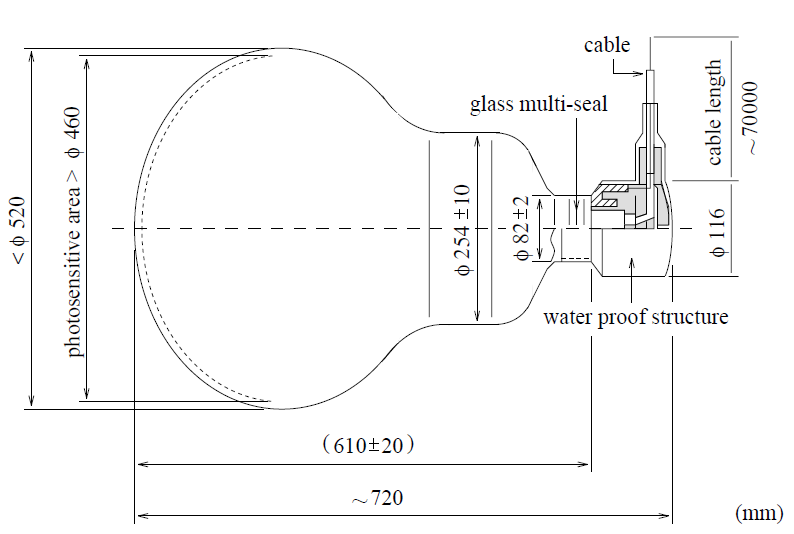
\includegraphics[width=0.8\textwidth]{Figures/PMT_schematic.png}
\caption{Schematic of an ID 50 cm Super-Kamiokande PMT \cite{fukuda_super-kamiokande_2003}.}
    \label{fig:PMTdiagram}
\end{figure}


Radioactivity from radon, uranium and thorium radioisotopes in the Super-Kamiokande tank water and radon in the surrounding air could provide a low energy background to measurements which should be negated. In low-energy analyses, such as the analysis in this thesis, this becomes an even more significant issue. Microbes present in the mine water also present a problem as they cause a reduction in the the light attenuation length. Therefore the water used in Super-Kamiokande has to undergo a purification process - the water used is continuously reprocessed at a rate of 30 tons $h^-1$ in a closed loop system, which is the same method used to purify the water when refilling the tank. The first step of this water purification process is to use a 1 $\micro m$ mesh filter to remove large particulates of impurities from the water \cite{fernandez_status_2016}. A heat exchanger is then used to cool down the water to a constant 13.0 \degree C to reduce the dark noise hits of the photomultiplier tubes and the growth of the microbes. A treatment with ultraviolet light is then used to kill any remaining microbes in the water. Radon-free air is then dissolved into the water to aid in the later process of radon removal from the water and a high performance membrane ultra filter (UF) is used to remove organic compounds about 10 nm in diamater from the water. After this step a membrane degasifier removes the dissolved radon, where 30 L of radon reduced air is supplied to the membrane degasifier. The dissolved radon will transfer across the membrane but the water will not, allowing for efficient radon reduction. 
\newline 

The inner detector tank water is circulated by injecting the water at the bottom of the tank and exctracting it from the top, where the convection currents are able to maintain the temperature in the region within 11 m to the bottom of tank, however, outside this region the present temperature gradient causes an asymmetry in the attenuation of light, which is discussed more in Chapter 3. 
\newline
 An air purification system is also installed in Super-Kamiokande in order to reduce the amount of Radon present which could dissolve into the tank and affect measurements. The level of radon activity achieved after this air purification has taken place is 1 mBq/$m^{3}$.

The Super-Kamiokande experiment began taking data on 1st April 1996, and due to maintenance was shut down in July 2001, which was phase I of the experiment. A table of the Super-Kamiokande phases is shown in Table \ref{table:phasetable}. During the refilling of the tank after maintenence, there was cascade of PMT implosions that occurred on the 12th of November 2001, which were triggered by the implosion of a single photomultiplier tube, due to a microfracture in the neck of the tube. This implosion destroyed about 7,000 of the PMTs and in order to avoid such chain reactions in the future, from 2002 onwards all of the inner detector PMTs are fitted with acrylic covers and fiber-glass reinforced plastic (FRP) cases. Detector shutdown and rebuild took nine months and Super-Kamiokande resumed data taking with the full number of photomultiplier tubes in July 2006 which marked the beginning of Super-Kamiokande phase III. Super-Kamiokande phase IV began in September 2008 where a new data aquisition system and charge to time (QTC) based electronics with Ethernet (QBEE) was deployed in order to measure arrival times and integrated charge for inner detector and outer detector photomultiplier tube signals. This replaced the ATM (Analogue and Timing Module). The improvements in electronics and calibration methods meant that when Super-Kamiokande phase IV started running in September of 2008, electrons with energies as low as 3.5 MeV were able to be detected.

\begin{table}[htp]
    $$
\begin{array}{|c|c|c|c|c|c|c|}
    
    \hline \multirow{2}{*}{\text { Phase }} & \multirow{2}{*}{\text { Phase Period }} & \multicolumn{2}{|c|}{\text { Total PMT number  }} & \multirow{2}{*}{\text { FRP case? }} & \multirow{2}{*}{\text { Readout }} & \multirow{2}{*}{\text { Gd\% }} \\
    \tabularnewline
    \cline {3-4} & &  \text { ID (Coverage) } & \text { OD } & & \tabularnewline
    \hline \hline \text { SK-I } & \text { Apr. 1996 - Jul. 2001 } & 11146(40 \%) & 1884 & \text { no } & \text { ATM } & 0 \\
    \hline \text { SK-II } & \text { Oct. 2002 - Oct. 2005 } & 5182(19 \%) & 1884 & \text { yes } & \text { ATM } & 0 \\
    \hline \text { SK-III } & \text { Jul. 2006 - Sep. 2008 } & 11129(40 \%) & 1884 & \text { yes } & \text { ATM } & 0 \\
    \hline \text { SK-IV } & \text { Sep. 2008 - May 2018 } & 11129(40 \%) & 1884 & \text { yes } & \text { QBEE } & 0 \\
    \hline \text {SK-V} & \text{ Jan. 2019 - Jul. 2020 }    &  11129(40 \%) & 1884 & \text { yes } & \text { QBEE } & 0 \\
    \hline \text {SK-VI} & \text{ Aug. 2020 - May 2022 }    &  11129(40 \%) & 1884 & \text { yes } & \text { QBEE } & 0.01\% \\
    \hline \text {SK-VII} & \text{ Jun. 2022 - Today }    &  11129(40 \%) & 1884 & \text { yes } & \text { QBEE } & 0.03\% \\
    \hline \hline 
\end{array}
    $$
\caption{Phases of Super-Kamiokande and main properties of each phase }
\label{table:phasetable}
\end{table}



\subsection{Data aquisition system}

As shown in Table \ref{table:phasetable}, Phase IV of the experiment marked the beginning of Super-Kamiokande using QTC-based Electronics with Ethernet (QBEEs). Each QBEE board used in Super-Kamiokande contains 24 photomultiplier tube input channel, where each channel uses a charge-to-time (QTC) converter and a time-to-digital converter placed in series as shown in Figure \ref{fig:superkdaq}. After a single photoelectron is produced by the photomultiplier tubes after incident photons have been recieved upon it, the dynodes inside the photomultiplier tube amplify this photoelectron so that each photoelectron that strikes the surface of the dynode produces several more photoelectrons, which are produced from the dynodes as an analogue signal. This signal then enters a charge-to-time converter (QTC), an application specific integrated circuit (ASIC) which was specifically designed for Super-Kamiokande in order to detect photomultiplier tube signals using built-in discriminators and to produce output timing signals whose widths represent the integrated charge of the PMT signal. The QTC used has three input channels per chip, which has three gain ranges (Small, Medium, Large as shown in Figure \ref{fig:superkdaq}). There is a built in discriminator inside the QTC which determines whether the the signal from a PMT is a ``hit". If the PMT signal exceeds the threshold value of this discriminator, the QTC integrates the charge of the signal over the next 400 ns, and a square wave pulse is generated whose pulse width is proportional to the intergrated charge of the input signal from the PMT. The next ~400 ns is used to discharge the integrated charge from the QTC, leading to a total channel dead time of 900 ns due to summing the charge integration and discharge of the QTC. 
\newline

\begin{figure}
    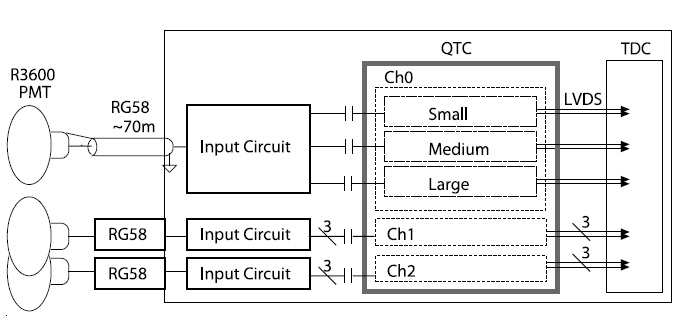
\includegraphics[width=\textwidth]{Figures/superk_daq.png}
\caption{Schematic of the charge-to-time converter circuit \cite{nishino_high-speed_2009}.}
    \label{fig:superkdaq}
\end{figure}

A time-to-digital converter (TDC) then digitises the output time signal, so the PMT charge information is retained. These digitised outputs are collated by 20 front-end computers which collects all the information from the inner and outer detectors, with each computer taking the PMT hit information from 30 inner detector and 20 outer detector QBEE boards and sorting the PMT hit time information in order of the raw hit time. This information is then sent to ``merger" computers, who then produce a full time-ordered list of all PMT hits. These merger computers then apply software triggers to select event candidates, using $N_{200}$, a quantity which determines the number of PMT hits in a 200 ns timing window. When the value of $N_{200}$ surpasses the threshold value of a certain trigger type (whether it is a SLE (Super Low Energy), LE (Low Energy), HE (High Energy), SHE (Super High Energy), OD (Outer Detector) or AFT (After Window) trigger), the trigger is used to select an event candidate. The SLE, LE, HE and SHE triggers roughly define the energy of a certain event, based on the number of hits detected. The OD trigger is used to veto events, and the AFT trigger is of special importance to the analysis in this thesis: it is used to discern when a neutron is produced after a neutrino interaction. The AFT Trigger is issued to take 500 $\mu$sec of data after SHE trigger in order to identify the positron from the prompt event and the delayed 2.2 MeV gamma released from the neutron capture on the proton during the IBD reaction. Another set of computers acts as an ``organiser": it takes all the information regarding the event candidates from the ``merger" computers and writes them onto disks \cite{fukuda_super-kamiokande_2003}.


\section{Event Reconstruction}

\subsection{Vertex Reconstruction}
For low energy events (events up to 100 MeV), Super-Kamiokande currently uses BONSAI (Branch Optimisation Navigating Successive Annealing Interactions) for event reconstruction. Vertex reconstruction for Super-Kamiokande has undergone changes and improvements depending on the phase of the experiment. 
\newline{}
For Phase I of Super-Kamiokande, vertex reconstruction depended on a lattice of test vertices with 4 m spacing throughout the detector, with a specific measure of goodness for each test vertex: the test vertex with the highest measure of goodness would have around it a more finely spaced grid, and the process would be repeated. For Phase II of Super-Kamiokande due to the reduced number of PMTs, this approach was no longer as successful as it was in Phase I and as a result the reconstruction perfomance declined, and BONSAI was created as a replacement. Instead of using a fixed grid which was the case with SK-I and SK-II, BONSAI creates test vertices by selecting groups of four PMT hits and seeing where the timing residuals of the PMT hits would be most reduced. After these test vertices have been indentified, a maximum likelihood fit over all the PMT hits in the event is performed, shown in Equation \ref{bonsailikelihood}.

\begin{equation}
    \mathcal{L}(\vec{x}, t_{0})=\sum_{i=1}^{N_{\text {hlt }}} \log (P(t-t_{\text {tof }}-t_{0}))
\label{bonsailikelihood}
\end{equation}

where ($\vec{x}, t_{0}$) is the test vertex, and $(P(t-t_{\text {tof }}-t_{0}))$ (shown in Figure \ref{fig:bonsaihittof}) is the probablility density function of the timing residual, which for each PMT hit is defined as $(t-t_{\text {tof }}-t_{0})$, where $t_{0}$ is the time of the interaction, $t_{tof}$ is the time of flight from the interaction vertex position to the position of the hit PMT, $t$ is the PMT hit time. The 1$\sigma$ difference between the true vertex position and the reconstructed vertex position plotted as a function of true electron energy is shown in Figure \ref{fig:bonsaivertexres}. 

\begin{figure}
    \centering
    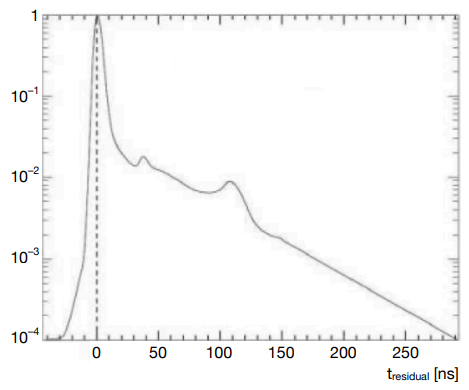
\includegraphics[width=0.8\textwidth]{Figures/bonsai_pdf_res.png}
\caption{Probability density of the timing residual P$(t-t_{\text {tof }}-t_{0})$, where $t_{0}$ is used for the vertex reconstruction maximum likelihood fit. The peaks at 30ns and 100ns are caused by PMT after-pulsing.}
    \label{fig:bonsaihittof}
\end{figure}

\begin{figure}
    \centering
    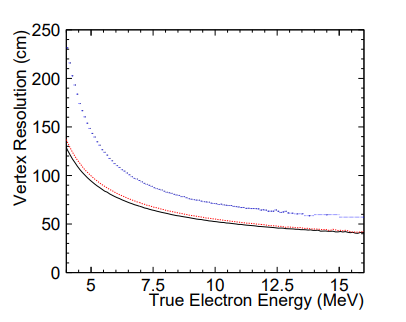
\includegraphics[width=0.8\textwidth]{Figures/bonsai_vertex_res.png}
\caption{The vertex resolution (the point at which 68\% of the events in the distance distribution between the actual and reconstructed vertex are contained) for the different SK phases. SK-I (Blue), SK-III (Red), SK-IV (Black).}
    \label{fig:bonsaivertexres}
\end{figure}

\subsection{Direction Reconstruction}

Cherenkov light is emitted in a conical formation as electrons and positrons travel through water, with a Cherenkov angle of $\approx 42\degree$. BONSAI can reconstruct the direction of these particles by using this information along with the reconstructed vertex. This reconstruction occurs using a maximum likelihood function defined in Equation \ref{eq:directionlikelihoodeq}.

\begin{equation}
    \mathcal{L}(\vec{d})=\sum_{i}^{N_{20}} \log (f(\cos\theta_{i}, E))\times\frac{\cos\theta_{i}}{a(\theta_{i})}
    \label{eq:directionlikelihoodeq}
\end{equation}

The term $f(\cos\theta_{i},E)$ in Equation \ref{eq:directionlikelihoodeq} is the expected distribution of the angle between the vector of the direction $\vec{d}$ of the particle, and the observed Cherenkov photon from the position of the reconstructed vertex. The reason there is a spread in this energy distribution is because while the highest value of this distribution occurs at the cosine of the opening Cherenkov angle of $42\degree$, due to the particle travelling through the water being Coulomb scattered multiple times, there is a variation in the angle because of the varying particle energy. The term $N_{20}$ is the number of hits whose residual hit time is within 20 ns of the time of the reconstructed event, which is used in order to reduce the amount dark noise and scattered photons contribute to the direction reconstruction calculation. The variable $a(\theta_{i})$ is a correction factor stemming from the acceptance of PMTs and therefore linked to the shape of the PMT and its acrylic case, is linked to the angle of incidence of the photon on the PMT, and is related to the angle of incidence of the photon on the PMT.


\subsection{Energy reconstruction}

The kinetic energy of a particle is proprtional to the amount of Cherenkov photons emitted from it, and if we assume that the Cherenkov photons in a single event come from a single electron, we can reconstruct the total energy of the electron. Instead of using the number of photoelectrons of all hit photomultiplier tubes to reconstruct the energy of low energy events, the number of hit photomultiplier tubes is used instead. The reasons for this are threefold - firstly, low energy events emit a small number of Cherenkov photons, and therefore average about one photon per hit PMT. Secondly, at single photoelectron level, the resolution of the PMTs is poor, and third, the number of photoelectrons produced is related to the gain of the PMT.
\newline
Due to the variation in gain value not affecting the number of hit photomultiplier tubes as much as it does for the number of photoelectrons, number of hit PMTs is used instead. To reduce dark noise, energy reconstruction uses $N_{50}$, which is the number of time of flight corrected photomultiplier tube hits in a 50 ns window. The number of effective photomultiplier tubes which are hit in this timing window of 50 ns are summed up, while being weighted with correction factors, to give $N_{eff}$ shown in Equation \ref{eq:effectivePMTs} \cite{ueno_analysis_nodate}. 

\begin{equation}
    N_{e f f}=\sum_{i=1}^{N_{50}}\left[\left(X_{i}-\epsilon_{\text {dark }}+\epsilon_{\text {tail }}\right) \times \frac{N_{\text {all }}}{N_{\text {alive }}} \times \frac{1}{S\left(\theta_{i}, \phi_{i}\right)} \times \exp \left(\frac{r_{i}}{\lambda}\right) \times G(i)\right]
\label{eq:effectivePMTs}
\end{equation}

where $X_{i}$ is the correction factor hits with many photoelectrons. This correction factor is important because if some photomultiplier tubes are hit by multiple photons (for example, if the edge of the fiducial volume is where the event vertex took place). The number of photoelectrons produced by each hit photomultiplier tube is estimated using the occupancy of the eight photomultiplier tubes which surround it. Using the number of hit photomultiplier tubes ($n_{i}$) and the number of functional photomultiplier tubes that surround the i-th photomultiplier tube ($N_{i}$), the formula for $X_{i}$ is shown in Equation \ref{eq:correction_factor}.

\begin{equation}
    X_{i}=\left\{\begin{array}{ll}
    \log \left(1-n_{i} / N_{i}\right)^{-N_{i} / n_{i}} & \left(n_{i}<N_{i}\right) \\
    3 & \left(n_{i}=N_{i}\right)
    \end{array}\right.
    \label{eq:correction_factor}
\end{equation}


The term $\epsilon_{dark}$ in Equation \ref{eq:correction_factor} is a correction factor for dark noise hits, shown in Equation \ref{edark}, where $R_{dark}$ is the average value for the dark rate during the run period that the event is in and $N_{\text {PMT}\text {alive }}$ is the number of active photomultiplier tubes in the inner detector.


\begin{equation}
    \epsilon_{\text {dark }}=\frac{N_{\text {PMT}\text {alive }} \times R_{\text {dark }} \times 50 \mathrm{~ns}}{N_{50}}
    \label{edark}
\end{equation}

The term $\epsilon_{tail}$ is the correction factor for photomultiplier tube hits which are in the tail end of the 50ns timing window, and is defined in Equation $\ref{etail}$.

\begin{equation}
    \epsilon_{\text {tail }}=\frac{N_{100}-N_{50}-N_{\text {alive }} \times R_{\text {dark }} \times(100-50) \mathrm{ns}}{N_{50}}
    \label{etail}
\end{equation}


The term $\frac{1}{S(\theta_{i}, \phi_{i})}$ is the inverse of the effective area of the ith hit photomultiplier tube photocathode, from the direction of the incident photon given by it's solid angle $(\theta_{i}, \phi_{i})$.

$G(i)$ is the gain correction for the quantum efficiency of the photomultiplier tubes and $exp(\frac{r_{s}}{\lambda})$ is the correction for water transparency which accounts for the amount of attenuation undergone by the photons in water, where $\lambda$ is the water transparency measured during the run period which includes the event, and $r_{i}$ is the distance between the reconstructed event vertex and the i-th hit PMT.

The average of each $N_{eff}$ distribution is taken, after producing multiple $N_{eff}$ distributions with fixed energies using Monte Carlo. These energies are fitted with a polynomial which is a function of the averaged $N_{eff}$ distribution, so the reconstructed energy is converted from $N_{eff}$.

\section{Super-Kamiokande Gadolinium Upgrade}

In order to be able to observe the diffuse supernova neutrino background (DSNB) flux it was proposed that Gadolinium (Gd) should be added to the the water in Super-Kamiokande. There are two natural isotopes of gadolinium, Gd-155 and Gd-157, which have large thermal neutron capture cross sections of 60740 barns and 253700 barns respectively. As a result of this, when neutrons are captured on them there is a cascade of gamma rays that occurs, with an energy totalling ~8 MeV, whereas neutron capture that occurs on hydrogen produces a single 2.2 MeV gamma ray, as the thermal neutron capture cross-section of hydrogen is just 0.329 barns \cite{meo_measurement_nodate}.  The ultimate aim is to load a total amount of gadolinium in the form of gadolinium sulphate octahydrate ($
\mathrm{Gd}_{2}\left(\mathrm{SO}_{4}\right)_{3} \cdot 8 \mathrm{H}_{2} \mathrm{O}$) in Super-Kamiokande which equates to 0.2\% of Gd by mass, which would allow for 90\% neutron capture efficiency. The ability to tag neutrons efficiently in Super-Kamiokande will benefit multiple physics topics, not only for the aforementioned observation of DSNB flux, but also for analyses involving atmospheric neutrinos and proton decay. 

\subsection{The EGADS project}

In 2009, prior to the addition of gadolinium in Super-Kamiokande, the EGADS (Evaluating Gadolinium's Action on Detector Systems) project was used to evaluate how the inclusion of $\mathrm{Gd}_{2}\left(\mathrm{SO}_{4}\right)_{3} \cdot 8 \mathrm{H}_{2} \mathrm{O}$ would affect water quality and detector components inside Super-Kamiokande and their analyses, and also to test the water system circulation. Measurements regarding neutron tagging were also taken using an Americium/Beryllium (Am/Be) source placed inside EGADS. As shown in Figure \ref{eq:ambe_decay}, this is because it produces a prompt 4.4 MeV gamma ray alongside a neutron during its decay process, and as a result the prompt 4.4 MeV signal can serve as a trigger signal, while the following hundreds of microseconds can be used as a timing window within which to scan for the neutron. Due to its similarity to the neutral current quasieleastic events studied in the analysis in this thesis, it can serve as a helpful control sample and is used in the calculation of the detector response uncertainty in Chapter 7. 

\begin{equation}
\begin{array}{c}
\alpha^{9} \mathrm{Be} \longrightarrow^{12} \mathrm{C}^{*} \mathrm{n} \\
{ }^{12} \mathrm{C}^{*} \longrightarrow{ }^{12} \mathrm{C} \gamma(4.4 \mathrm{MeV})
\end{array}
\label{eq:ambe_decay}
\end{equation}

The delayed neutron capture time from an Am/Be source used in EGADS with the gadolinium sulphate concentration of 0.2\% is shown in Figure \ref{fig:EGADS_ambe_capture}. Here, we can see that the neutron capture time from the data is 29$\pm$0.3 $\mu$s and for the Monte Carlo it is 30$\pm$0.8 $\mu$s.

\begin{figure}[H]
    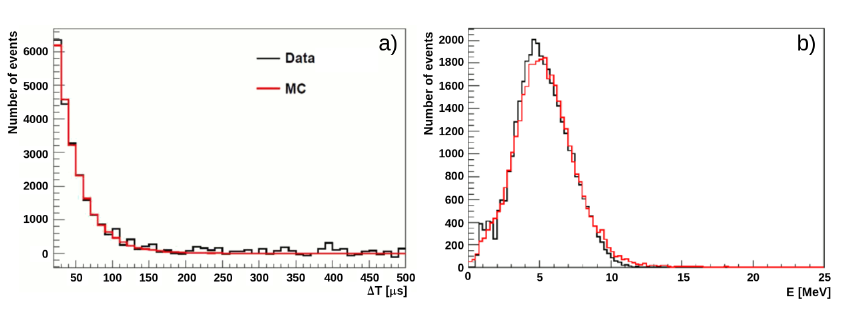
\includegraphics[width=\textwidth]{Figures/egads_ambe.png}
\caption{(a) Delayed neutron capture time from prompt event with Am/Be source. (b) Reconstructed energy from gamma rays after neutron capture.}
\label{fig:EGADS_ambe_capture}
\end{figure}


EGADS represented the most realistic possible soak test, and after two and a half years of running, EGADS was emptied in November 2017 to check the condition of the inner structure and the photomultiplier tubes. There was no deteriation of any of the components, which was an excellent sign for a detector designed to so closely resemble the conditions for the Super-Kamiokande Gadolinium upgrade. 

\subsection{Gadolinium loading into Super-Kamiokande}

After the success of EGADS, the Super-Kamiokande Gadolinium project was formed in 2015 with the final goal of adding 0.2\% $\mathrm{Gd}_{2}\left(\mathrm{SO}_{4}\right)_{3} \cdot 8 \mathrm{H}_{2} \mathrm{O}$ by mass to the detector. The first step of gadolinium loading began with the loading of 13 tons of $\mathrm{Gd}_{2}\left(\mathrm{SO}_{4}\right)_{3} \cdot 8 \mathrm{H}_{2} \mathrm{O}$ into Super-Kamiokande from July 14th to August 17th 2020, which is about 10\% of the target concentration. The work in this thesis focuses on this first Gd loading period, not the second loading period which began in late May of 2022. 

\subsubsection{The SK-Gd water system}

The SK-Gd water system was designed to dissolve $\mathrm{Gd}_{2}\left(\mathrm{SO}_{4}\right)_{3} \cdot 8 \mathrm{H}_{2} \mathrm{O}$ powder into the detector water, pass it through a ``pretreatement" system to remove contaminants from the water, and then to continously circulate it. The design for this treatment system was successfully tested in EGADS and involves treating this solution with ultraviolet light. Positively charged impurites dissolved in the solution (such as radium ions) and negatively charged impurities (such as uranium) are removed using a cation and anion exchange resins respectively, after which a UV steriliser removes bacteria which were introduced in the dissolving process. 

The acceptable background rate after the final value for Gd loading  was set to be less than double that of the background rate for when Super-Kamioknde ran with pure water. As a result, rigorous standards of cleanliness were set for the $\mathrm{Gd}_{2}\left(\mathrm{SO}_{4}\right)_{3} \cdot 8 \mathrm{H}_{2} \mathrm{O}$ powder, which meant setting maximum allowed levels of radioactive impurites which are shown in Table \ref{gdpowderradiation}.


\begin{table}[H]

    $$
    \begin{array}{llll}
    \hline \text { Chain } & \text { Isotope } & \text { Criterion [mBq/kg] } & \text { Physics target } \\
        \hline{ }^{238} \mathrm{U} & { }^{238} \mathrm{U} & <5 & \text { SRN } \\
    & { }^{226} \mathrm{Ra} & <0.5 & \text { Solar } \\
    \hline{ }^{232} \mathrm{Th} & { }^{232} \mathrm{Th} & <0.05 & \text { Solar } \\
    & { }^{228} \mathrm{Ra} & <0.05 & \text { Solar } \\
    \hline{ }^{235} \mathrm{U} & { }^{235} \mathrm{U} & <30 & \text { Solar } \\
    & { }^{227} \mathrm{Ac} /{ }^{227} \mathrm{Th} & <30 & \text { Solar } \\
    \hline
    \end{array}
    $$
\caption{Table of impurities in the gadolinium sulphate octahydrate powder}
\label{gdpowderradiation}
\end{table}

\subsubsection{SK-Gd attenuation, transparency and concentration monitoring}

After the loading of $\mathrm{Gd}_{2}\left(\mathrm{SO}_{4}\right)_{3} \cdot 8 \mathrm{H}_{2} \mathrm{O}$ into Super-Kamiokande, water transparency and attenuation length were continously monitored. This had also been conducted in EGADS (see previous section), but due to the flow rate of the water and method by which gadolinium is loaded into the detector being different in Super-Kamiokande, it is important to monitor these attributes in the SK-Gd upgrade as well. Figure \ref{fig:gdattenuationlength} shows how the attenuation length of the Cherenkov light in SK-Gd varies with time: this attenuation length is measured using cosmic ray through going muons (as explained in Chapter 3). There is a clear decrease in the attenuation length after the loading of $\mathrm{Gd}_{2}\left(\mathrm{SO}_{4}\right)_{3} \cdot 8 \mathrm{H}_{2} \mathrm{O}$, reaching a minimum of 75 m in August of 2020, and increasing again to its original pre-Gadolinium loading value of 90 m by the beginning of December 2020.  

\begin{figure}[H]
    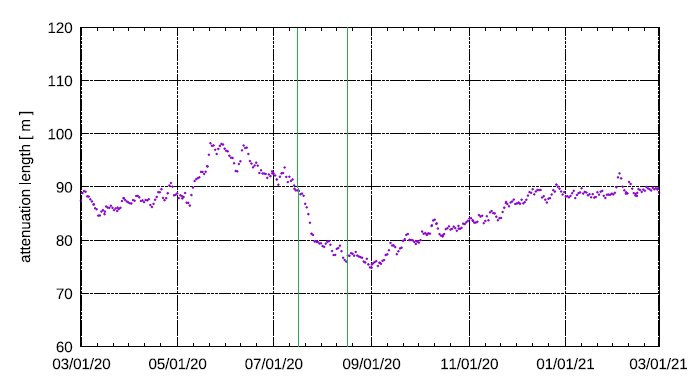
\includegraphics[width=\textwidth]{Figures/attenuation_length_gd.png}
    \caption{The attenuation length of Cherenkov light measured using cosmic ray muons between March of 2020 and March of 2021}
    \label{fig:gdattenuationlength}
\end{figure}

It is important to monitor the concentration of the $\mathrm{Gd}_{2}\left(\mathrm{SO}_{4}\right)_{3} \cdot 8 \mathrm{H}_{2} \mathrm{O}$ in the detector - this can be done using either direct sampling via calibration ports or using the Americium/Beryllium neutron source. Using a sampling probe and a conductivity meter to take samples in the inner and outer detector, the conductivity was measured. Figure \ref{fig:gdconductivity} shows the variation of the $\mathrm{Gd}_{2}\left(\mathrm{SO}_{4}\right)_{3} \cdot 8 \mathrm{H}_{2} \mathrm{O}$ concentration in the detector at different depths in the detector during various points in time in the gadolinium loading period. 

\begin{figure}[H]
    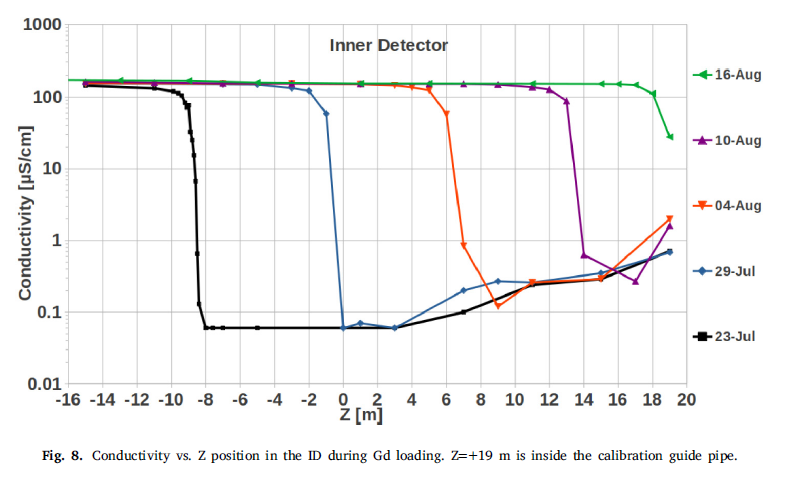
\includegraphics[width=\textwidth]{Figures/gd_conductivity.png}
    \caption{Conductivity vs. z position during Gd loading inside the inner detector}
    \label{fig:gdconductivity}
\end{figure}


By placing an Am/Be source into the inner detector of Super-Kamiokande using the central calibration port and then monitoring the source at three posiitons along the Z-axis, the concentration of $\mathrm{Gd}_{2}\left(\mathrm{SO}_{4}\right)_{3} \cdot 8 \mathrm{H}_{2} \mathrm{O}$ could be measured. One measurement position is in the middle of the detector (Z=0 m) and the other two were at Z = +12 and Z = -12 m respectively. By searching for neutron capture events on gadolinium from the Am/Be data, a time distribution of neutron capture candidates could be plotted and fit with a function shown in Figure \ref{fig:ambe_time}. The Am/Be source position here was Z=0 m and the 0 $\mu$s time value on the x-axis is the time at which the scintillation photons produced by the 4.4 MeV gamma ray from its passing through the BGO cube are detected. 


\begin{figure}[H]
    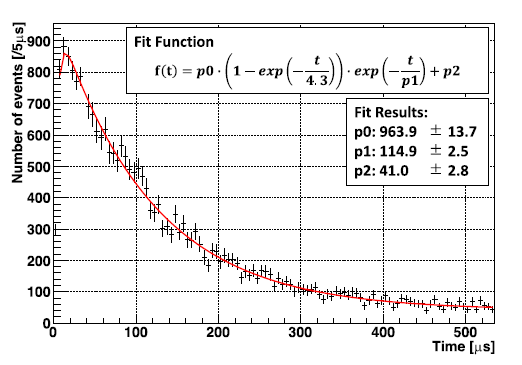
\includegraphics[width=\textwidth]{Figures/ambe_time.png}
    \caption{Neutron capture time distribution for the Am/Be source placed at Z=0 m.}
    \label{fig:ambe_time}
\end{figure}

Using GEANT4 Monte Carlo simulations, the neutron capture time could be converted to a value for Gd concentration, where a mean capture lifetime of $115 \pm 1$ \micro s corresponds to a Gd concentration value of $111 \pm 2$ ppm, consistent with the target concentration value of 0.011\%.


To summarise, Super-Kamiokande has undergone a lot of transformations over its lifetime, with modifications made to its data aquisition system and methods of event reconstruction with each successive new phase. The biggest change made to the detector is the upgrade to Super-Kamiokande Gd, where in the summer of 2020 0.026\% of $\mathrm{Gd}_{2}\left(\mathrm{SO}_{4}\right)_{3} \cdot 8 \mathrm{H}_{2} \mathrm{O}$ was added to the detector: a long-awaited next step which would enhance sensitivity to the detection of neutrons emitted in inverse beta decay compared to that in water.

















